% ISPRS 2026 Abstract — 2-page limit
\documentclass{isprs}
\usepackage{subfigure}
\usepackage{setspace}
\usepackage{geometry}
%\usepackage{epstopdf}
\usepackage[labelsep=period]{caption}
\usepackage[british]{babel}
\usepackage[hang]{footmisc}
\usepackage{graphicx}
\usepackage{booktabs}
\usepackage{float}
\usepackage{amsmath}
\def\footnotemargin{1em}

\geometry{a4paper, top=25mm, left=20mm, right=20mm, bottom=25mm, headsep=10mm, footskip=12mm}
\captionsetup{justification=centering,font=normal}
\captionsetup[figure]{font=small}
\captionsetup[table]{font=small}

\begin{document}

\title{Integrating Multi-View Stereo and Depth Foundation Models\\for Precise 3D Reconstruction of Thin Urban Structures}

\author{Hwiyoung Kim\textsuperscript{1}, Impyeong Lee\textsuperscript{2}}

\address{
	\textsuperscript{1 }Geospatial Team, InnoPAM, Yongsan-gu, Seoul, Korea -- hykim@innopam.com\\
	\textsuperscript{2 }Dept.\ of Geoinformatics, University of Seoul, Dongdaemun-gu, Seoul, Korea -- iplee@uos.ac.kr\\
}

\keywords{3D Reconstruction, Multi-View Stereo, Monocular Depth Estimation, Depth Foundation Model, Thin Structures, Power Lines}
\maketitle

\sloppy

\section{Introduction}\label{sec:intro}

High-fidelity urban Digital Twins require geometrically accurate 3D models of all constituent objects. Standard Structure-from-Motion (SfM) and Multi-View Stereo (MVS) pipelines~\cite{schonberger2016sfm} remain the industry standard for producing metric 3D reconstructions from multi-view imagery, yet they systematically fail on thin, texture-less structures such as power lines: stereo matching failure produces depth map voids that are filled by interpolation from background surfaces during mesh generation.

To address thin structure reconstruction, implicit neural representations such as NeRF~\cite{mildenhall2021nerf} and 3D Gaussian Splatting~\cite{kerbl2023gaussian} achieve visually compelling results but lack the explicit metric surface definitions required for surveying applications. Meanwhile, recent Monocular Depth Estimation (MDE) foundation models---including ZoeDepth~\cite{bhat2023zoedepth}, Depth Anything~V2~\cite{yang2024dav2}, and Marigold~\cite{ke2024marigold}---predict dense, structurally coherent depth from single images, including thin structures, but lack absolute metric scale. Prior Depth Anything~\cite{wang2025priorda} fuses sparse metric points with MDE through a learned alignment network, but its fixed internal resolution (518$\times$518) causes thin structures to vanish.

We propose a hybrid pipeline that combines MVS metric accuracy with MDE structural completeness for thin structure reconstruction. Our approach is grounded in two empirical findings: (1)~MDE models estimate wire depth close to pole depth in relative space, enabling metric scale propagation; and (2)~high-resolution patch-based MDE~\cite{li2024patchfusion} is essential to preserve 2--3\,pixel-wide structures.

\section{Method}\label{sec:method}

\textbf{Stage~1: MVS Depth with Hole Identification.}
SfM/MVS processing produces per-image metric depth maps and camera poses. Thin structures exhibit systematic depth voids (Table~\ref{tab:results}, ``MVS only'').

\textbf{Stage~2: High-Resolution MDE.}
PatchFusion~\cite{li2024patchfusion} with Depth Anything~V1 processes images at native 8192$\times$5460 resolution via tile-based inference (\texttt{patch\_split\_num}=[7,8]). A pilot study confirmed wire--pole relative depth ratio~$<$~0.3 across three test images (Table~\ref{tab:results}).

\textbf{Stage~3: Scale-Aware Fusion and Refinement.}
MVS valid pixels are retained. For invalid pixels (thin structure voids), MDE relative depth is calibrated to metric scale using pole regions as anchors: an affine transform $d_{\text{metric}} = s \cdot d_{\text{rel}} + t$ is estimated via RANSAC at pole locations (radius\,=\,300\,px). Wire-like structures are identified by Sobel edge detection with morphological closing and aspect ratio filtering ($>$\,5). Each wire group receives a representative metric depth (median of RANSAC inliers within pole depth\,$\pm$\,5\,m). Multi-view joint optimisation refines wire 3D positions by minimising calibrated depth--projected depth residuals across adjacent views.

\section{Experiments}\label{sec:results}

\begin{figure*}[!t]
\begin{center}
	\includegraphics[width=0.95\textwidth]{figures/fig1_3d_reconstruction.png}
	\caption{3D reconstruction result of the fused pipeline. Red points indicate reconstructed power lines filled by calibrated MDE depth; green points denote utility poles with MVS-derived metric depth. Background buildings (blue) retain original MVS depth values. Oblique view demonstrates wire--building depth separation.}
	\label{fig:reconstruction}
\end{center}
\end{figure*}

We used 180 drone images (8192$\times$5460, DJI) of Seongsu-dong, Seoul, processed with Agisoft Metashape for SfM/MVS. Three images containing visible poles and wires were selected for detailed evaluation. Completeness was measured as the fraction of valid depth pixels in a 7$\times$7 patch at annotated wire/pole/background locations.

\begin{table}[h]
	\centering
	\small
	\begin{tabular}{@{}lcccc@{}}
		\toprule
		& \multicolumn{3}{c}{Completeness (\%)} & Wire depth \\
		\cmidrule(lr){2-4}
		Method & Wire & Pole & Bkgd & (m) \\
		\midrule
		MVS only     & 0--8  & 59--100 & 62--100 & --- \\
		MDE only     & 100   & 100     & 100     & (relative) \\
		Fused (Ours) & 100   & 100     & 100     & 64.26 \\
		\midrule
		\multicolumn{4}{@{}l}{Pole MVS depth (reference)} & 65.46 \\
		\multicolumn{4}{@{}l}{Background MVS depth} & 69.47 \\
		\bottomrule
	\end{tabular}
	\caption{Depth completeness and metric accuracy. Wire depth of our method (64.26\,m) is within 1.2\,m of pole depth (65.46\,m), confirming wire\,$\approx$\,pole\,$<$\,background.}
	\label{tab:results}
\end{table}

\textbf{Quantitative Results.}
Table~\ref{tab:results} summarises the key metrics. MVS achieves 0--8\% completeness at wire locations versus 59--100\% at poles. Our fused result fills all wire voids while retaining MVS values at valid pixels. The fused wire depth (64.26\,m) is 1.2\,m from the pole MVS depth (65.46\,m) and 5.2\,m closer than the background (69.47\,m), confirming the wire\,$\approx$\,pole\,$<$\,background relationship. Multi-view joint optimisation reduced per-view calibration residuals to 0.13--0.33\,m.

\textbf{Ablation: Depth Profile at Wire Location.}
Figure~\ref{fig:profile} shows the vertical depth profile crossing a wire (x\,=\,4734 in image 0656). MVS depth is absent at the wire (y\,=\,2925--2938). The calibrated MDE profile shows a depth dip at the wire pixel (y\,$\approx$\,2933), consistent with pole depth. The fused result preserves this structure. At y\,=\,2941, MVS resumes at 79.17\,m (background building), demonstrating clear wire--background separation.

\textbf{Limitations.}
PatchFusion's tile-based processing introduces inter-patch relative scale inconsistency: pixels at the same MVS depth (66\,m) exhibited MDE values ranging from 5.7 to 12.2 depending on image position. This limits the accuracy of affine scale transfer and necessitates local, pole-anchored fitting. Edge-based wire detection produced discontinuous groups, and inter-view 3D discrepancy reached 3.25\,m before joint optimisation.

\begin{figure}[H]
\begin{center}
	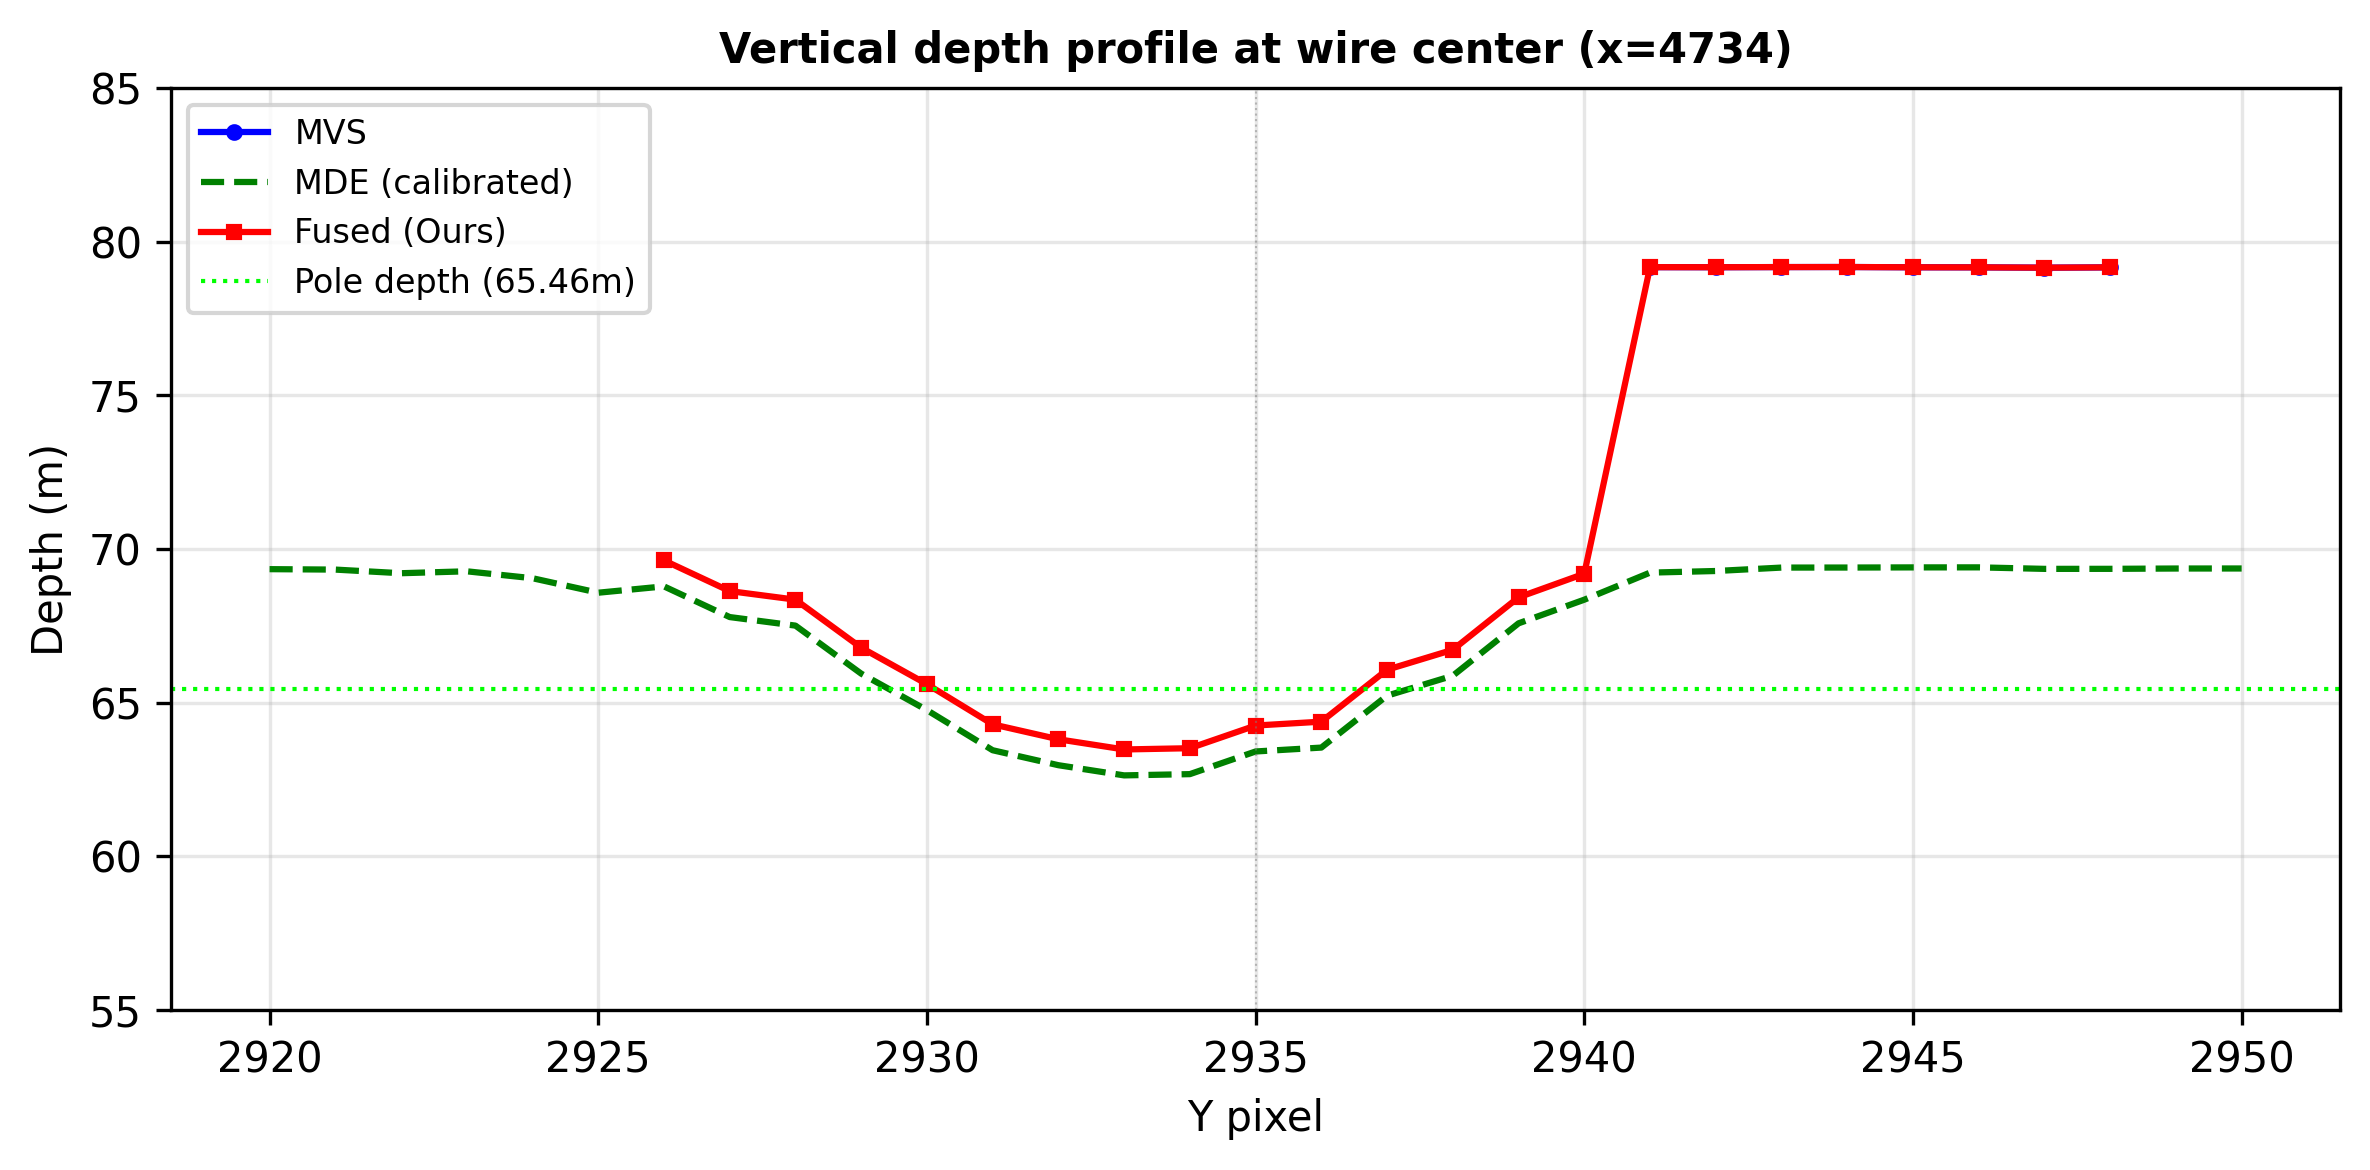
\includegraphics[width=0.95\columnwidth]{figures/fig2_profile.png}
	\caption{Ablation: vertical depth profile at wire centre (x\,=\,4734). MVS (blue) has no values at the wire. Calibrated MDE (green, dashed) and fused result (red) show wire depth near pole reference (65.46\,m, dotted line). At y\,=\,2941, MVS resumes at 79\,m (background).}
	\label{fig:profile}
\end{center}
\end{figure}

\section{Conclusion}\label{sec:conclusion}

We presented a pipeline for reconstructing thin urban structures by fusing MVS metric depth with MDE structural completeness. Our analysis established that MDE foundation models estimate wire depth close to pole depth in relative space, enabling metric scale transfer without domain-specific physical priors. High-resolution MDE (PatchFusion, 8K) was essential for preserving structures only 2--3\,pixels wide. Current limitations include MDE inter-patch scale inconsistency and wire detection fragmentation. Future work will focus on multi-view consistent scale estimation and learned thin-structure segmentation.

\section*{Acknowledgements}
This work is supported by the Korea Agency for Infrastructure Technology Advancement (KAIA) grant R&D program of Digital Land Information Technology Development funded by the Ministry of Land, Infrastructure and Transport (MOLIT) (Grant RS-2022-00142501).

{
	\begin{spacing}{1.17}
		\normalsize
		\bibliography{ISPRSguidelines_authors}
	\end{spacing}
}

\end{document}
